\section{Discussion}\label{Discussion}

A main motivation for this work is the emergence of seemingly unique representations from sparse coding models trained on natural data, despite the varied assumptions underlying the many algorithms in current use. Our results constitute an important step toward explaining these phenomena as well as unifying many publications on the topic by deriving general deterministic conditions under which identification of parameters in this model is not only possible but also robust to uncertainty in measurement and model choice.

We have shown that, given sufficient data, the problem of determining a dictionary and sparse codes with minimal support size (Prob.~\ref{OptimizationProblem}) reduces to an instance of Prob.~\ref{InverseProblem}, to which our main result (Thm.~\ref{DeterministicUniquenessTheorem}) applies: every dictionary and sequence of sparse codes consistent with the data are equivalent up to inherent relabeling/scaling ambiguities and a discrepancy (error) that scales linearly with the measurement noise or modeling inaccuracy. The constants we provide are explicit and computable; as such, there is an effective procedure that sufficiently affirms if a proposed solution to these problems is indeed unique up to noise and inherent ambiguities, although it is not efficient in general.

%A compelling feature of this model is its simple instantiation of the principle of Occam's razor: a natural video, for instance, is modeled as a linear combination of a small number of spatiotemporal building blocks, each representing an archetypical feature latent in the data. 

%For theoretical neuroscience in particular, dictionary learning and related methods have recovered characteristic components of natural images \cite{Olshausen96, hurri1996image, bell1997independent, van1998independent} and sounds \cite{bellsejnowski1996, smithlewicki2006} that reproduce response properties of certain cortical neurons.  

%to the recovery of ``mouse neuronal activity representing location on a track \cite{agarwal2014spatially}

%Moreover, we show that even if the meta-parameter for the number of dictionary elements is overestimated, a subset of parameters may still be identifiable up to noise. 

Beyond an extension of existing noiseless guarantees \cite{Hillar15} to the noisy regime and their novel application to Prob.~\ref{OptimizationProblem}, our work contains a theory of combinatorial designs for support sets key to identification of dictionaries. We incorporate this idea into a fundamental lemma in matrix theory (Lem.~\ref{MainLemma}) that draws upon the definition of a matrix lower bound (\ref{Ldef}) induced by a hypergraph. The new insight offered by this combinatorial approach allows for guaranteed recovery of some or all dictionary elements even if: 1) dictionary size is overestimated, 2) data cover only a polynomial number of distinct sparse supports, and 3) dictionaries do not satisfy the spark condition. 

The absence of any assumptions about dictionaries solving Prob.~\ref{InverseProblem} was a major technical obstruction in proving Thm.~\ref{DeterministicUniquenessTheorem}. We sought such a general guarantee because of the practical difficulty in ensuring that an algorithm maintain a dictionary satisfying the spark condition \eqref{SparkCondition} at each iteration, an implicit requirement of all previous works except \cite{Hillar15}; indeed, even certifying a dictionary has this property is NP-hard \cite{tillmann2014computational}.

One direct application of this work is to theoretical neuroscience, wherein our theorems justify the mathematical soundness of one of the few hypothesized theories of bottleneck communication in the brain \cite{Isely10}: that sparse neural population activity is recoverable from its noisy linear compression through a randomly constructed (but unknown) wiring bottleneck by any biologically plausible unsupervised sparse coding method that solves Prob.~\ref{DeterministicUniquenessTheorem} or \ref{SLCopt} (e.g., \cite{rehnsommer2007, rozell2007neurally, pehlevan2015normative}).\footnote{We refer the reader to \cite{ganguli2012compressed} for more on interactions between dictionary learning and neuroscience.}

In fact, uniqueness guarantees with minimal assumptions apply to all areas of data science and engineering that utilize learned sparse structure. For example, several groups have applied compressed sensing to signal processing tasks; for instance, in MRI analysis \cite{lustig2008compressed}, image compression \cite{Duarte08}, and even the design of an ultrafast camera \cite{Gao14}. It is only a matter of time before these systems incorporate dictionary learning to encode and decode signals (e.g., in a device that learns structure from motion \cite{kong2016prior}), just as scientists have used sparse coding to make sense of their data \cite{jung2001imaging, agarwal2014spatially, lee2016sparse, wu2016stability}. 

Assurances offered by our theorems certify that different devices and algorithms learn equivalent representations given enough data from statistically identical systems.\footnote{To contrast with the current hot topic of ``Deep Learning'', there are few such uniqueness guarantees for these models of data; moreover, even small noise can dramatically alter their output \cite{goodfellow2014explaining}.} 
Indeed, a main reason for the sustained interest in dictionary learning as an unsupervised method for data analysis seems to be the assumed well-posedness of parameter identification in the model, confirmation of which forms the core of our findings.

\section{Future Directions}

There are many challenges left open by this work. All conditions stated here guaranteeing the uniqueness and stability of sparse representations have only been shown sufficient; it remains open, therefore, to extend them to necessary conditions, be they on required sample size, the structure of support set hypergraphs, or tolerable error bounds. On this last note, we remark that the deterministic conditions derived here must consider always the ``worst-case" noise, whereas the ``effective" noise sampled from a concentrated distribution might be significantly reduced, especially for high-dimensional data. It would be of great practical benefit to see how drastically all conditions can be relaxed by requiring only probabilistic guarantees in this way, or in the spirit of our discussion on probabilistic pigeonholing to reduce sample complexity (as in the famous ``birthday paradox") following the proof of Thm.~\ref{DeterministicUniquenessTheorem}.

Another interesting question raised by this work is for which special cases is it efficient to check that a solution to Prob.~\ref{InverseProblem} or \ref{OptimizationProblem} is unique up to noise and inherent ambiguities. Considering that the sufficient conditions we have described for checking this in general are NP-hard to compute, are the necessary conditions hard? Are Probs.~\ref{InverseProblem} and \ref{OptimizationProblem} then also hard (e.g., see \cite{Tillmann15})? Finally, since Prob.~\ref{SLCopt} is intractable in general, but efficiently solvable by $\ell_1$-norm minimization when the matrix is known (and has a large enough lower bound over sparse domains \cite{eldar2012compressed}), is there a version of Thm.~\ref{SLCopt} certifying when Prob.~\ref{OptimizationProblem} can be solved efficiently in full by similar means?  % [*** Incorporate this open problem with more words ***]

We hope these remaining challenges pique the interest of the community to pick up where we have left off and that the theoretical tools showcased here may be of use to this end.



%We close with some challenges left open by our work. First, there is the basic problem of proving optimal lower bounds on sufficient sample size $N$ guaranteeing the uniqueness and stability of sparse representations. The pigeonholing argument in the proof of Thm.~\ref{DeterministicUniquenessTheorem} is loose in that it assigns to each support $S \in \mathcal{H}$ a corresponding support $\overline S$ without consideration of previously matched pairs; although we doubt tightening in this way will lead to sub-exponential sample sizes. Sample complexity will also benefit from lowering the number of required supports, i.e. the size of regular uniform hypergraphs satisfying the SIP. The regularity requirement on support hypergraphs can be loosened to allow for certain non-regular hypergraphs satisfying constraints on the degree sequence of nodes; though we impose regularity for clarity of exposition. It is then natural to ask: what is the smallest hypergraph satisfying the required constraints forgiven $m$ and $k$? Finally, the error bounds can be improved by tightening the constant $C_1$, e.g. via an improvement in Lemma ?.

%Solving Prob.~\ref{SLCopt} directly is intractable in general since it necessitates, for each proposed dictionary $\mathbf{B}$, a combinatorial search for the supports of the associated sparse codes $\mathbf{\overline x}_i$. A common work-around is to convexify the problem (for fixed $\mathbf{B}$) by substituting the norm $\|\cdot\|_0$ with $\|\cdot\|_1$, impelled the fact that matrices $\mathbf{A}$ with large enough $L_{2k}(\mathbf{A})$ induce the same sparse codes via minimization of either norm \cite{?}. To this end, the lower bound $L_{2k}(\mathbf{BP}) \geq (L_{2k}(\mathbf{A}) - C_1\varepsilon) / \|\mathbf{D}\|_1$ implied by Thm.~\ref{DeterministicUniquenessTheorem} hints at conditions on the generating dictionary $\mathbf{A}$ and $k$-sparse codes $\mathbf{x}_i$ under which \emph{all} matrices $\mathbf{B}$ (of bounded column-norm) that solve Prob.~\ref{OptimizationProblem} also share this property of $\mathbf{A}$ by virtue of uniqueness and stability. One might then imagine an inference procedure whereby sparse codes are inferred via minimization of $\|\cdot\|_1$, but solutions still evaluated by their collective support size, yielding unique optimal solutions to Prob.~\ref{SLCopt} if only constraints could be imposed such that the learning procedure eventually guides $\mathbf{B}$ through an optimal dictionary. % (e.g. the dictionary is a member of a known finite set).

%\section{EXTRA}
%An additional consequence of Thm.~\ref{DeterministicUniquenessTheorem} of potential practical relevance to is the implied lower bound $L_{2k}(\mathbf{BPD}) \geq L_{2k}(\mathbf{A}) - C_1\varepsilon$ in the case where $\mathbf{A}$ satisfies \eqref{SparkCondition}. Since solving Prob.~\ref{SLCopt} directly requires a combinatorial search over sparse supports for the $\mathbf{\overline x}_i$ for each proposed dictionary $\mathbf{B}$, rendering it intractable in general, a common strategy is to replace the $\ell_0$-norm in \eqref{minsum} with the $\ell_1$-norm, thereby transforming the inference of sparse $\mathbf{\overline x}_i$ for a fixed dictionary $\mathbf{B}$ into a convex optimization solvable by a linear program. A major advance in compressive sensing was the discovery that, for fixed $\mathbf{B}$, solutions to \eqref{minsum} using either norm yield the same sparse vectors $\mathbf{\overline x}_i$ (up to noise) provided $L_{2k}(\mathbf{B})$ is large enough \cite{?}. What our results hint at are conditions on the generating dictionary $\mathbf{A}$ and $k$-sparse codes $\mathbf{x}_i$ under which \emph{all} matrices $\mathbf{B}$ (of bounded column-norm) that solve Prob.~\ref{OptimizationProblem} also share this property by virtue of uniqueness and stability; that is, conditions which guarantee that the sparse codes $\mathbf{\overline x}_i$ solving Prob.~\ref{OptimizationProblem} also solve the convexified problem when the corresponding dictionary $\mathbf{B}$ is held fixed. It remains to determine, however, what practical conditions preclude matrices that don't solve Prob.~\ref{OptimizationProblem} from nonetheless solving the convexified problem.
%
%Regardless, an implication of the above observation is that the following algorithm solves Prob.~\ref{OptimizationProblem} without appeal to combinatorial search:
%\begin{enumerate}
%\item List all matrices $\mathbf{B}$.
%\item For each matrix $\mathbf{B}$, solve $\mathbf{\overline x}_i = \arg \min \|\mathbf{v}\|_1$ s.t. $\|\mathbf{Bv} - \mathbf{z}_i\| \leq \eta$ for $i = 1, \ldots, N$.
%\item Quantify the proposed solution $\mathbf{B}$ and $\mathbf{\overline x}_1, \ldots, \mathbf{\overline x}_N$ as $\rho(\mathbf{B}, \mathbf{\overline x}_1, \ldots, \mathbf{\overline x}_N) = \sum_{i=1}^{N} \|\mathbf{\overline x}_i\|_0$.
%\item Output $\arg \min_{\mathbf{B}, \mathbf{\overline x}_1, \ldots, \mathbf{\overline x}_N} \left( \rho \right)$.
% \end{enumerate}


%Since its inception some twenty years ago, sparse coding has become a standard tool in signal analysis, yielding myriad insights into the structure of natural signals across a variety of scientific domains. In this work, 

%We make a final remark about the tightness of our results and the computability of our derived constants.
%We remark that our constants have been derived for deterministic ``worst-case'' noise, whereas the ``effective'' noise might be smaller when sampled from a distribution.

%Our results suggest that this correspondence could be due to the ``universality'' of sparse representations in natural data, an early idea in neural theory \cite{pitts1947}. 

% \vspace{-.2 cm}

%\showacknow % Display the acknowledgments section


%The problem is to count integer solution to the problem $\sum_i a_i = N$ subject to $a_i < i$ for all $i$. There is as far as [internet person] knows no closed formula for this general problem, but there is a formula that allows the number of solutions to be computed in a number of operations independent of ??. Consider first the case that all limits are equal ??1=??2=?=????=??. Then the number is the coefficient of ???? in the polynomial (1+??+?+????)??. By writing this as a rational function of ??...
%see:
%https://math.stackexchange.com/questions/553960/extended-stars-and-bars-problemwhere-the-upper-limit-of-the-variable-is-bounded

\begin{figure}\label{probpigeon}
\begin{center}
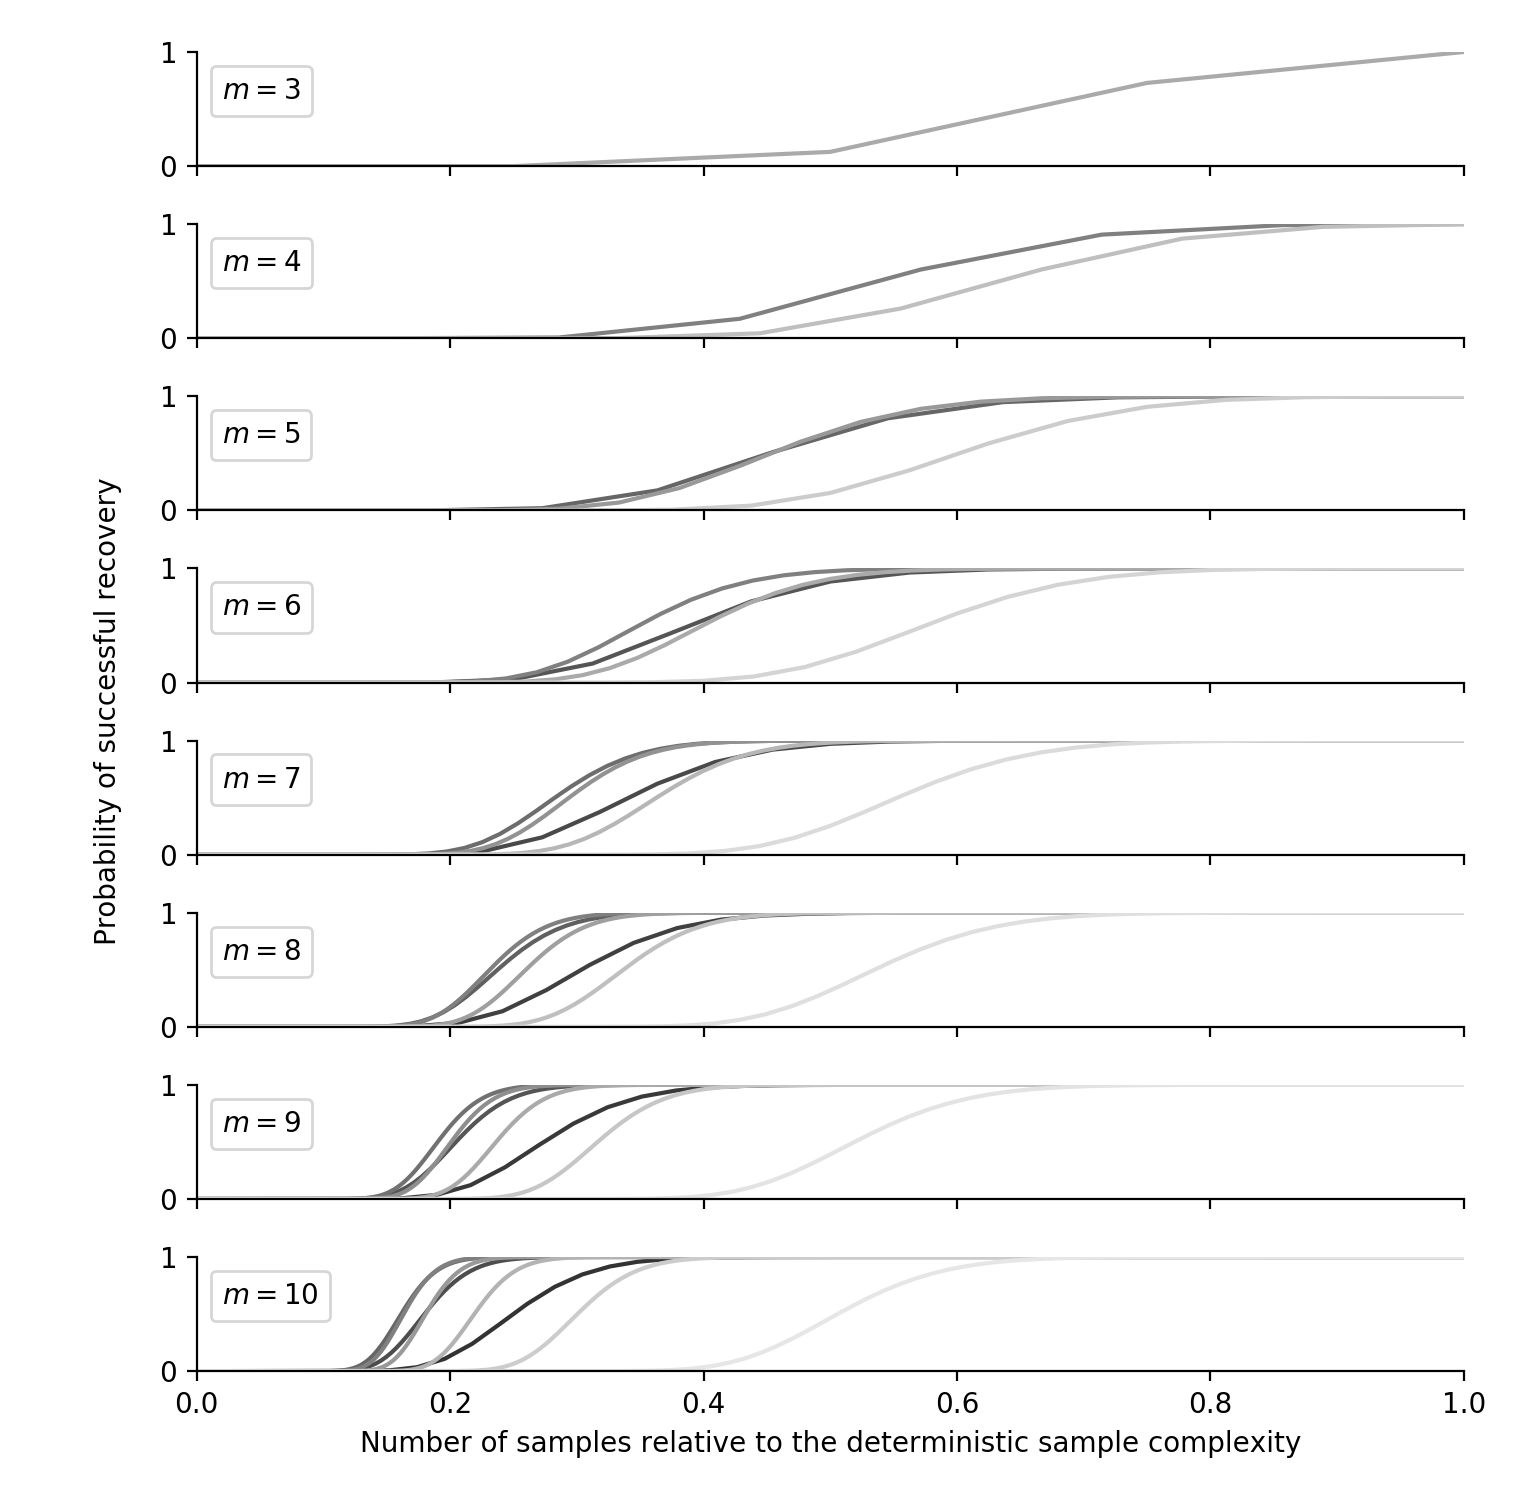
\includegraphics[width=1 \linewidth]{figures/prob_vs_samples.png}
\caption{Probability of successful dictionary and code recovery (as per Thm. \ref{DeterministicUniquenessTheorem}) for a number of samples $N$ given as a fraction of the deterministic sample complexity $N = |\mathcal{H}|[(k-1){m \choose k} + 1]$ when $\mathcal{H}$ is taken to be the set of $m$ consecutive intervals of length $k$ in a cyclic order on $[m]$ (i.e. $|\mathcal{H}|=m$). Successful recovery is nearly certain far below the deterministic sample complexity.}
\vspace{-.6 cm}
\label{probvsamples}
\end{center}
\end{figure}

\begin{figure}\label{reasonableC2}
\begin{center}
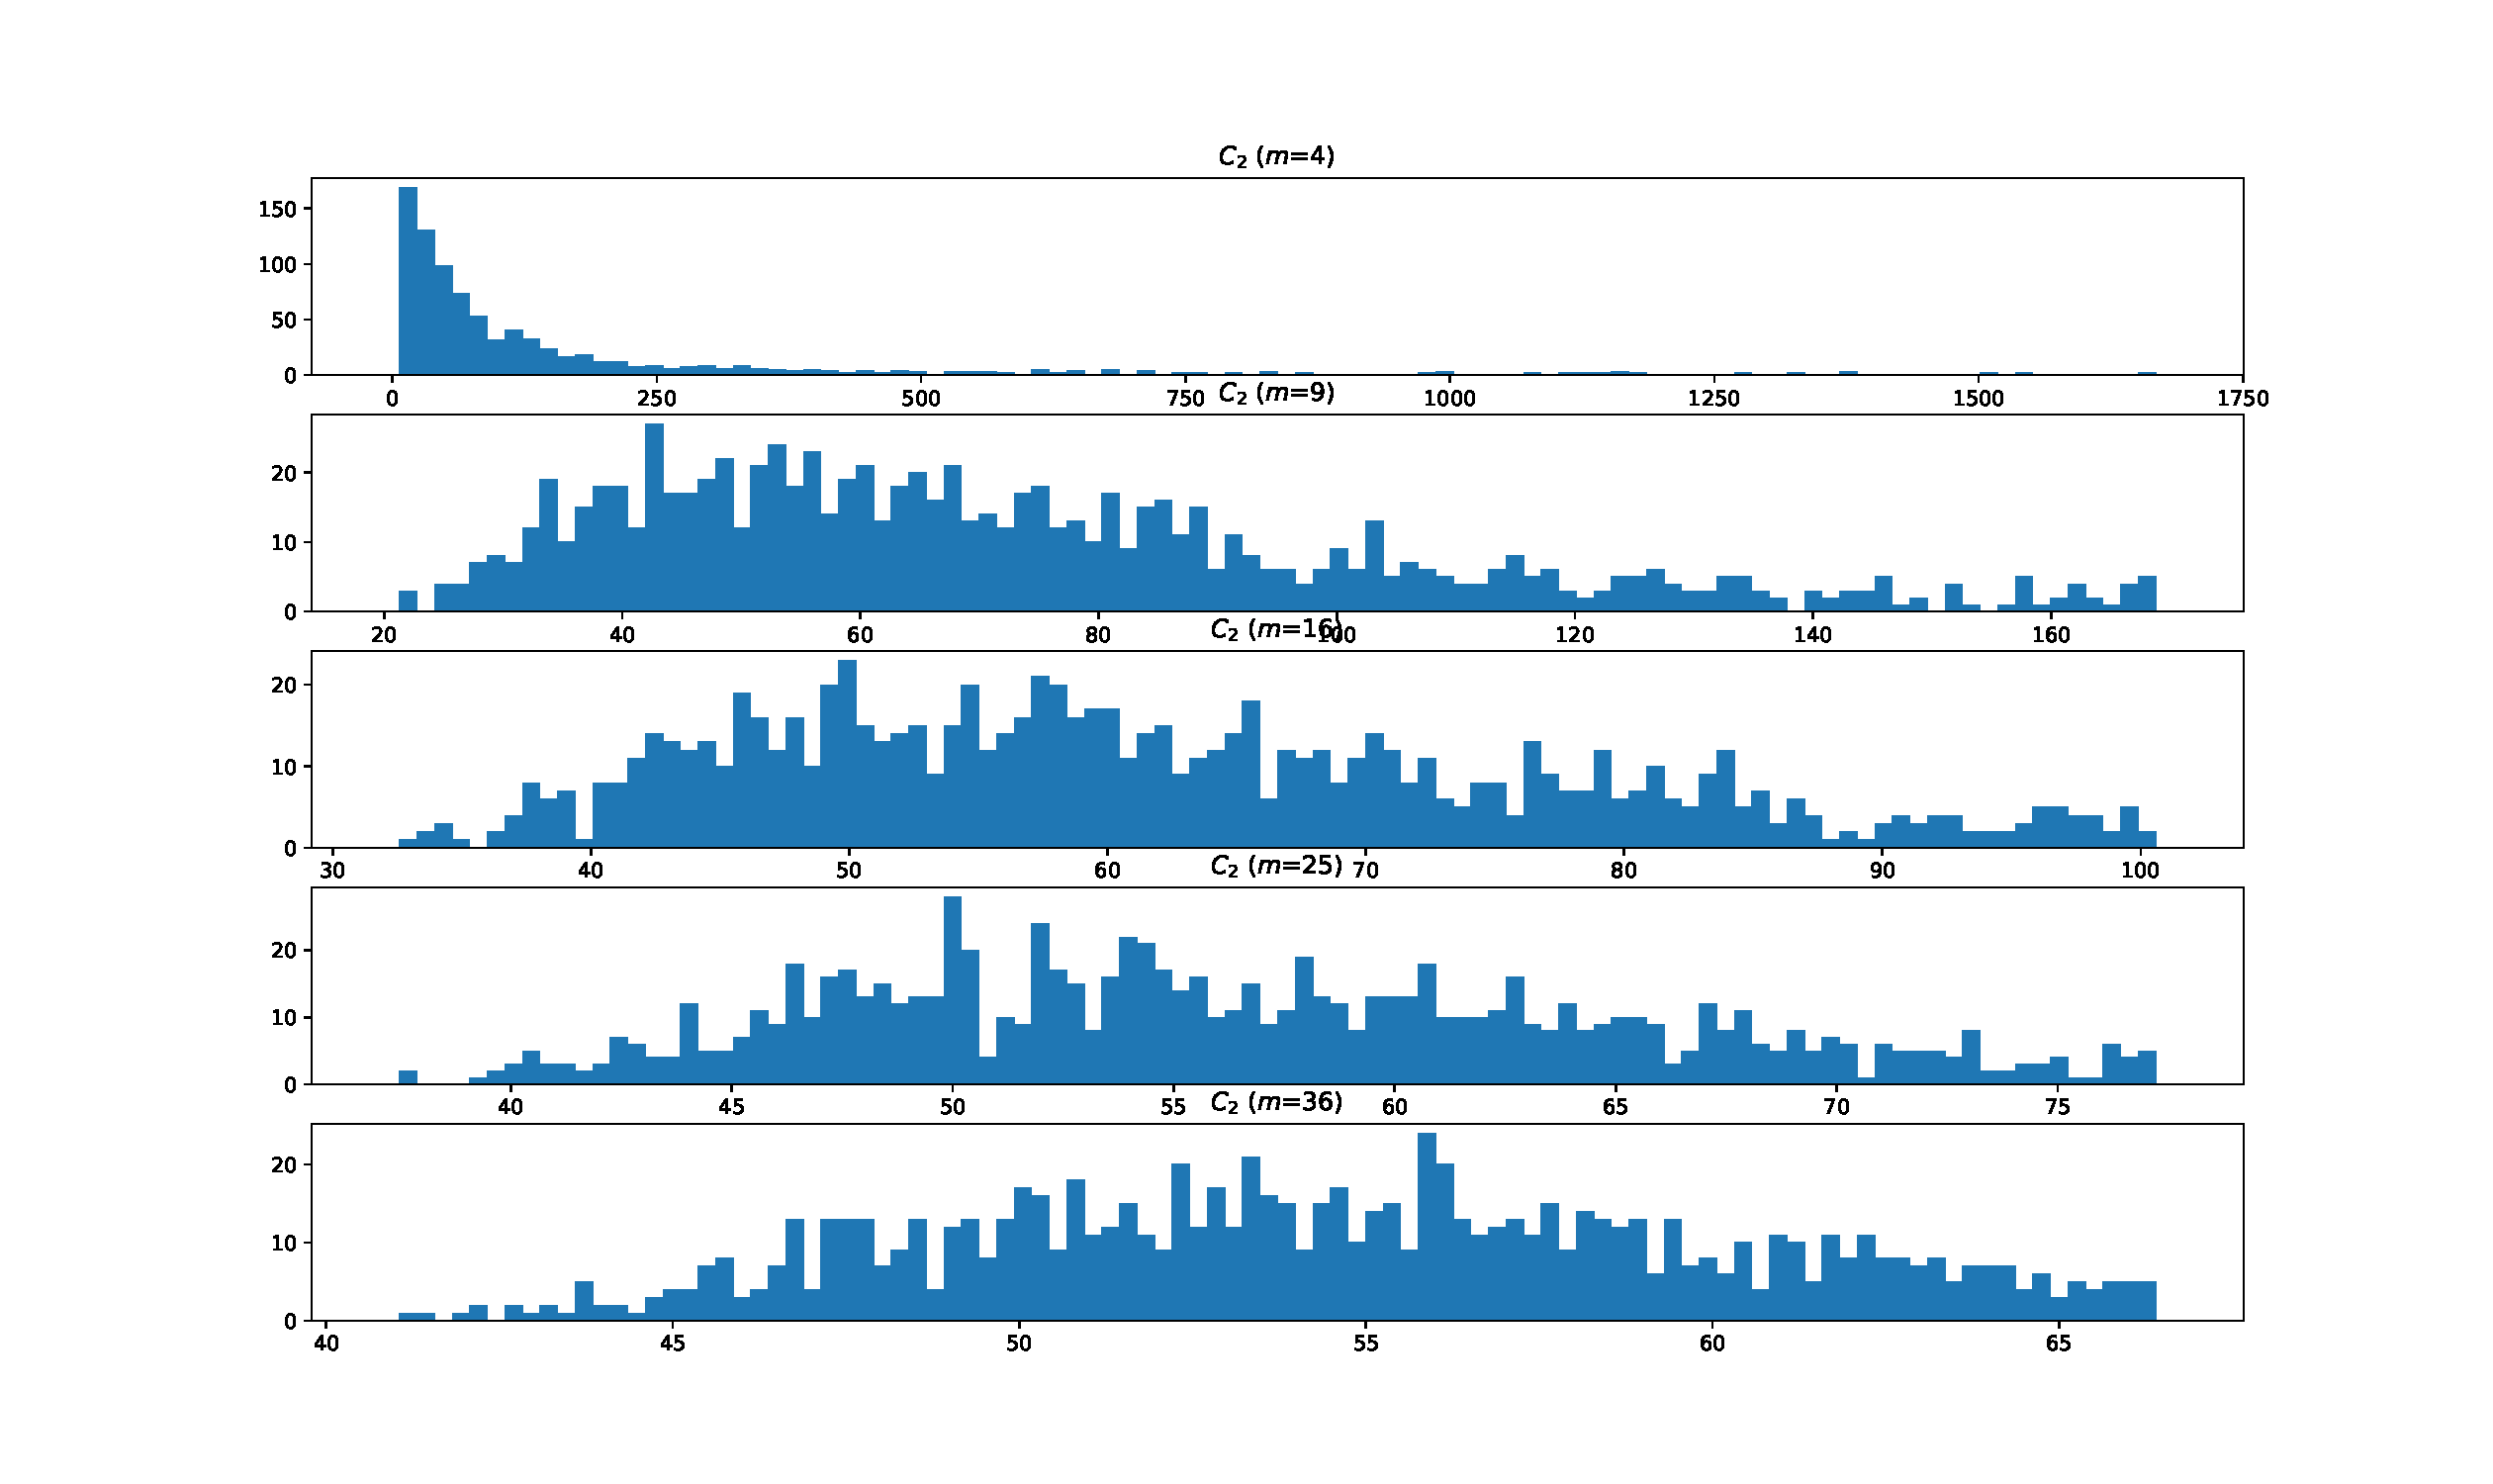
\includegraphics[width=1 \linewidth]{figures/C2_m36_nt1000.pdf}
\caption{The constant $C_2(\mathbf{A}, \mathcal{H})$ computed for generic unit-norm matrices $\mathbf{A} \in \mathbb{R}^{n \times m}$ and the hypergraph $\mathcal{H}$ consisting of the rows and columns formed by arranging  the elements of $[m]$ into a square grid. The results suggest that the bound is typically concentrated around a reasonable value.}
\vspace{-.6 cm}
\label{samples_vs_m}
\end{center}
\end{figure}


